\documentclass[journal]{IEEEtran}

\usepackage{amsmath,amsfonts,amssymb}
\usepackage{algorithmic}
\usepackage{graphicx}
\usepackage{textcomp}
\usepackage{xcolor}
\usepackage{booktabs}
\usepackage{cite}
\usepackage{url}
\usepackage{subcaption}

\begin{document}

\title{A Generalized Federated Learning Framework for Private Cross-Institutional Medical Diagnostics}

\author{Prof.~Rachana~G~Sunkad,
        Pavitra~Devendachar~Badiger,
        Prajwal~P~Raikar,
        Tejas~M~G,
        and~Vijeta~B~Muttagi%
\thanks{Prof. Rachana G Sunkad is an Assistant Professor with the Department of Computer Science and Engineering, Bapuji Institute of Engineering and Technology, Davanagere, India.}%
\thanks{Pavitra Devendachar Badiger, Prajwal P Raikar, Tejas M G, and Vijeta B Muttagi are with the Department of Computer Science and Engineering, Bapuji Institute of Engineering and Technology, Davanagere, India.}%
}

\markboth{IEEE Transactions on Medical Imaging,~Vol.~XX, No.~XX,~October~2026}%
{Sunkad \MakeLowercase{\textit{et al.}}: Generalized Federated Learning Framework for Cross-Institutional Medical Diagnostics}

\maketitle

\begin{abstract}
Pneumonia detection from chest X-ray radiographs is an essential task in automated computer-aided clinical diagnosis. However, training deep learning diagnostic models using medical images from geographically dispersed healthcare institutions introduces significant barriers concerning data privacy regulations, cross-site statistical heterogeneity, and clinical black-box opacity. This paper presents an end-to-end federated learning framework for binary pneumonia classification that combines an ImageNet-pretrained ResNet-50 architecture, proximal regularization via FedProx, Transport Layer Security (TLS) encrypted model transport, and Gradient-weighted Class Activation Mapping (Grad-CAM) for visual interpretability. The framework is deployed and validated across three distinct multi-institutional chest radiograph client datasets (Kaggle, Chittagong, and Bhopal), totaling 6,363 images (5,116 training/validation images and 1,247 held-out test images). To safeguard patient privacy, an automated Optical Character Recognition (OCR) de-identification pipeline masks visible patient demographic identifiers on scans prior to contrast-limited adaptive histogram equalization (CLAHE) preprocessing. Training across three federated communication rounds reveals that proximal regularization ($\mu = 0.01$) stabilizes optimization across uneven sample distributions. On pooled multi-center test evaluation, the round-3 global model achieved an accuracy of 81.40\%, precision of 86.25\%, recall of 80.20\%, and F1-score of 83.11\%. A detailed client-level breakdown exposes domain-shift discrepancies across sites, illustrating that pooled evaluation alone can mask site-specific recall deficits. Visual explanations via Grad-CAM demonstrate that the model targets anatomically relevant pulmonary opacities, providing actionable interpretability for healthcare workflows.
\end{abstract}

\begin{IEEEkeywords}
Federated Learning, Pneumonia Detection, Chest X-Ray, ResNet-50, FedProx, Grad-CAM, Explainable Artificial Intelligence, Medical Privacy.
\end{IEEEkeywords}

\section{Introduction}
\IEEEPARSTART{P}{neumonia} continues to be one of the foremost causes of infectious morbidity and mortality worldwide, especially among pediatric and elderly populations \cite{wang2017chestxray8}. Diagnostic confirmation routinely relies on chest radiography (X-ray). However, the accurate interpretation of pulmonary infiltrates, consolidations, and bronchopneumonic opacities requires substantial radiological expertise, which remains constrained in resource-limited and rural medical facilities.

Recent developments in deep convolutional neural networks (CNNs) have shown remarkable capabilities in automating chest radiograph analysis, reaching expert radiologist benchmarks under controlled conditions \cite{rajpurkar2017chexnet, irvin2019chexpert}. Conventional deep learning approaches necessitate pooling massive quantities of patient radiographs into a unified central server. In clinical reality, centralized data aggregation is strictly restricted by privacy frameworks such as HIPAA \cite{hipaa1996, hhs2003} and GDPR \cite{gdpr2016}, alongside proprietary institutional data ownership concerns.

Federated Learning (FL) has emerged as an attractive decentralized machine learning paradigm \cite{mcmahan2017communication, kairouz2021advances, rieke2020future}. Rather than transmitting sensitive patient images to an external cloud, participating hospitals (clients) train diagnostic models on their local storage infrastructure. Only numerical parameter weights or gradients are communicated to an aggregation coordinator. Nevertheless, clinical federated learning encounters non-trivial real-world hurdles:
\begin{enumerate}
    \item \textbf{Statistical Heterogeneity (Non-IID Data):} Institutional datasets naturally vary in radiographic hardware calibration, acquisition protocols, patient demographics, and prevalence of pneumonia \cite{li2020federated}. Standard Federated Averaging (FedAvg) often experiences weight divergence under such skew.
    \item \textbf{Data Privacy in Transit:} Gradient exchanges across public networks remain susceptible to eavesdropping and gradient-inversion attacks \cite{zhu2019deep}, necessitating cryptographically secured communication.
    \item \textbf{Identifiable Information in Raw Scans:} Legacy hospital imaging systems frequently imprint patient names and hospital tags directly onto DICOM/radiograph pixels, risking privacy leaks even during local processing.
    \item \textbf{Explainability and Interpretability:} Black-box clinical predictions cannot be audited by medical practitioners without spatial verification of lesion focus \cite{selvaraju2017gradcam}.
\end{enumerate}

To overcome these challenges, this study presents a generalized federated learning diagnostic system developed and validated on three distinct real-world datasets: Kaggle, Chittagong Medical College Hospital, and Bhopal Memorial Hospital. The major contributions of this work are summarized as follows:
\begin{itemize}
    \item An automated privacy-preserving diagnostic pipeline is established, incorporating OCR-based text de-identification to strip embedded patient identifiers, followed by CLAHE contrast enhancement and ResNet-50 transfer learning.
    \item Federated optimization is conducted using FedProx with proximal parameter $\mu = 0.01$ to stabilize gradient convergence across statistically divergent client partitions.
    \item Transport Layer Security (TLS) mutual authentication is configured to protect model parameter transit between local clients and the central aggregation coordinator.
    \item Comprehensive global pooled and per-client evaluations are conducted across 3 communication rounds, highlighting critical trade-offs between precision and recall under non-IID conditions.
    \item Explainable Artificial Intelligence (XAI) is integrated using Grad-CAM, enabling visual localization of predictive lung regions for clinical verification.
\end{itemize}

\section{Related Work}
\subsection{Deep Learning for Chest Radiography}
Automated pneumonia classification using deep neural networks has advanced through residual learning architectures \cite{he2016deep} and large-scale public datasets \cite{wang2017chestxray8, irvin2019chexpert}. Rajpurkar et al. \cite{rajpurkar2017chexnet} established that transfer learning on DenseNet and ResNet models allows networks to recognize complex parenchymal opacities. However, models trained exclusively on single-institution distributions frequently experience severe generalization drops when deployed on external institutional cohorts.

\subsection{Decentralized and Federated Learning in Medicine}
Federated learning allows distributed healthcare nodes to collaboratively train a shared architecture while maintaining strict data governance \cite{sheller2019multi, sheller2020federated, kaissis2020secure, li2024federated}. McMahan et al. \cite{mcmahan2017communication} introduced Federated Averaging (FedAvg), aggregating client models proportionally to sample count. However, clinical data heterogeneity (non-IID) poses optimization challenges. Li et al. \cite{li2020federated} introduced FedProx, adding a quadratic proximal penalty to the local loss function to limit deviation from the global model checkpoint.

\subsection{Explainability in Medical AI}
Explainability is a prerequisite for clinical adoption. Selvaraju et al. \cite{selvaraju2017gradcam} proposed Gradient-weighted Class Activation Mapping (Grad-CAM), which calculates the gradients of the target class score with respect to feature maps in the final convolutional layer, producing coarse localization heatmaps of suspicious pathologies.

Table~\ref{tab:related_work} positions our framework in comparison to contemporary federated medical imaging literature.

\begin{table*}[t]
\centering
\caption{Comparison of Existing Approaches in Federated Medical Imaging}
\label{tab:related_work}
\begin{tabular}{llll}
\toprule
\textbf{Work} & \textbf{Application / Target} & \textbf{Core Methodology} & \textbf{Key Characteristics} \\
\midrule
Zhou et al. (2026) \cite{zhou2026federated} & Medical Image FL Benchmark & FL Benchmarking Suite & Comprehensive cross-dataset multi-benchmark. \\
Ali et al. (2026) \cite{ali2026privacy} & Multi-Institutional Data Mining & Privacy-Preserving FL & Evaluates cryptographic privacy tradeoffs. \\
Wagner et al. (2026) \cite{wagner2026feasibility} & Brain MRI Classification & Heterogeneous Client FL & Multi-disease evaluation under non-IID conditions. \\
Liu et al. (2026) \cite{liu2026new} & Medical Image Classification & One-Shot Rectified Flow & Communication-efficient one-shot distillation. \\
Latif et al. (2025) \cite{latif2025explainable} & Brain Tumor Diagnosis & Explainable FL (XAI) & Grad-CAM integration with federated client updates. \\
Usharani et al. (2025) \cite{usharani2025fedlres} & Lung Cancer Radiographs & ResNet-50 Federated Learning & Decentralized feature extraction on pulmonary CT. \\
Guleria et al. (2025) \cite{guleria2025fedpneu} & Multi-Client Pneumonia FL & Hybrid Proximal FL & Parameter-efficient client adaptation on X-rays. \\
\textbf{Present Work} & \textbf{Pneumonia Classification} & \textbf{ResNet-50 + FedProx + TLS + Grad-CAM} & \textbf{Full pipeline: OCR de-identification, TLS encryption,} \\
 & & & \textbf{FedProx optimization, pooled/client-wise audit, XAI.} \\
\bottomrule
\end{tabular}
\end{table*}

\section{System Architecture}
The framework comprises four core operational tiers: client data de-identification and preprocessing, local client optimization, TLS-encrypted orchestration, and explainable post-hoc auditing.

\subsection{Client-Side OCR De-Identification and Preprocessing}
Certain public or archival medical datasets (e.g., Client 2 / Chittagong) retain burned-in patient banners displaying name, age, and scan date. Before training, each radiograph is scanned with an Optical Character Recognition (OCR) model. Detected text boxes above confidence $\tau = 0.30$ are masked with zero-valued bounding boxes, preventing spurious shortcut learning.

Each image is subsequently enhanced using Contrast Limited Adaptive Histogram Equalization (CLAHE) to amplify lung parenchymal textures, resized to $224 \times 224 \times 3$, and normalized to standard ImageNet distribution vectors ($\mu = [0.485, 0.456, 0.406]$, $\sigma = [0.229, 0.224, 0.225]$).

\subsection{Local Model Architecture}
A deep convolutional ResNet-50 architecture \cite{he2016deep} is deployed across all clients. The original 1000-class fully connected output layer is replaced with a binary classification head:
\begin{equation}
\hat{y} = \sigma\left(W_{\text{fc}} \cdot \phi(x) + b_{\text{fc}}\right)
\end{equation}
where $\phi(x) \in \mathbb{R}^{2048}$ represents the global average pooled feature representation extracted from the final bottleneck block (\texttt{layer4}), and $\hat{y} \in \{0, 1\}$ corresponds to NORMAL and PNEUMONIA classes.

\subsection{FedProx Optimization and TLS Coordination}
During communication round $t$, the central coordinator distributes the global model checkpoint $w_t$. Each client $k \in \{1, 2, 3\}$ initializes its weights with $w_t$ and minimizes the FedProx local objective function:
\begin{equation}
F_k(w; w_t) = \mathcal{L}_k(w) + \frac{\mu}{2} \|w - w_t\|_2^2
\label{eq:fedprox}
\end{equation}
where $\mathcal{L}_k(w)$ is the cross-entropy classification loss over local dataset $\mathcal{D}_k$, and $\mu = 0.01$ penalizes local weight drift. Parameters are transmitted over mutually authenticated TLS connections using X.509 root CA certificates and RSA private keys.

\section{Materials and Methods}

\subsection{Multi-Institutional Dataset Composition}
The empirical setup employs three client datasets reflecting cross-institutional variation:
\begin{itemize}
    \item \textbf{Client 1 (Kaggle / Guangzhou Women and Children's Medical Center):} 2,683 training samples and 624 testing samples.
    \item \textbf{Client 2 (Chittagong Medical College Hospital):} 320 training samples and 110 testing samples. Contains burned-in patient demographic text.
    \item \textbf{Client 3 (Bhopal Memorial Hospital):} 2,113 training samples and 513 testing samples.
\end{itemize}
The global experimental corpus comprises 6,363 radiographs (5,116 training/validation and 1,247 held-out test images), as detailed in Table~\ref{tab:dataset_distribution}. For local model monitoring, each client dynamically holds out a reproducible 20\% validation subset from its training partition using fixed seed 42.

\begin{table}[h]
\centering
\caption{Distribution of Chest Radiographs Across Federated Clients}
\label{tab:dataset_distribution}
\begin{tabular}{lcccc}
\toprule
\textbf{Client Source} & \textbf{Training} & \textbf{Testing} & \textbf{Total} & \textbf{Class Balance (Normal / Pneu.)} \\
\midrule
Client 1 (Kaggle)     & 2,683 & 624 & 3,307 & 1,341 / 1,342 (Train) \\
Client 2 (Chittagong) & 320   & 110 & 430   & 160 / 160 (Train) \\
Client 3 (Bhopal)     & 2,113 & 513 & 2,626 & 1,063 / 1,050 (Train) \\
\midrule
\textbf{Total}        & \textbf{5,116} & \textbf{1,247} & \textbf{6,363} & \textbf{2,564 / 2,552 (Train)} \\
\bottomrule
\end{tabular}
\end{table}

\subsection{Hyperparameter Setup}
Training parameters were standardized across all participating clients to guarantee synchronous convergence, summarized in Table~\ref{tab:hyperparameters}.

\begin{table}[h]
\centering
\caption{Federated Experimental Training Configuration}
\label{tab:hyperparameters}
\begin{tabular}{ll}
\toprule
\textbf{Parameter} & \textbf{Value / Specification} \\
\midrule
Backbone Network           & ResNet-50 (ImageNet Pretrained) \\
Input Resolution          & $224 \times 224 \times 3$ \\
Batch Size                & 16 \\
Local Epochs per Round    & 3 \\
Communication Rounds      & 3 \\
Optimization Algorithm    & FedProx ($\mu = 0.01$) \\
Client Optimizer          & AdamW ($\text{lr} = 5 \times 10^{-5}$, weight decay $= 10^{-4}$) \\
Data Augmentation         & Random Horizontal Flip ($p=0.5$), Random Rotation ($5^\circ$) \\
Gradient Clipping         & Max norm $= 5.0$ \\
Network Encryption        & Transport Layer Security (TLS/X.509) \\
Evaluation Hardware       & Multi-Core CPU Environment \\
\bottomrule
\end{tabular}
\end{table}

\subsection{Performance Metrics}
Model quality is assessed on the held-out test partitions using Accuracy, Precision, Recall, and F1-score:
\begin{equation}
\text{Accuracy} = \frac{TP + TN}{TP + TN + FP + FN}
\end{equation}
\begin{equation}
\text{Precision} = \frac{TP}{TP + FP}, \quad \text{Recall} = \frac{TP}{TP + FN}
\end{equation}
\begin{equation}
\text{F1-Score} = \frac{2 \cdot \text{Precision} \cdot \text{Recall}}{\text{Precision} + \text{Recall}}
\end{equation}
where $TP$, $TN$, $FP$, and $FN$ represent true positive, true negative, false positive, and false negative counts, respectively. The positive class represents PNEUMONIA.

\subsection{Grad-CAM Visual Attribution}
To calculate class activation maps, the gradient of the predicted pneumonia score $y^c$ with respect to feature map $A^k$ of \texttt{layer4} is computed. Feature map weights $\alpha_k^c$ and heatmap $L_{\text{Grad-CAM}}^c$ are derived as:
\begin{equation}
\alpha_k^c = \frac{1}{HW} \sum_{i=1}^H \sum_{j=1}^W \frac{\partial y^c}{\partial A_{i,j}^k}
\end{equation}
\begin{equation}
L_{\text{Grad-CAM}}^c = \text{ReLU}\left(\sum_k \alpha_k^c A^k\right)
\end{equation}
The 2D heatmap is resized to $224 \times 224$ and superimposed onto the original radiograph.

\section{Experimental Results and Discussion}

\subsection{De-Identification and Preprocessing Results}
Medical imaging collected from historical hospital archives often contains burned-in metadata (e.g., patient name, scan date, institution identifier) directly visible on the radiograph canvas. Figure~\ref{fig:deidentification} illustrates a representative chest radiograph from Client 2 (Chittagong) before and after our automated EasyOCR de-identification procedure. The optical character recognition system identifies bounding regions around textual annotations and sets their pixel values to zero, ensuring patient anonymity and preventing the convolutional neural network from exploiting non-biological textual shortcuts.

\begin{figure}[t]
\centering
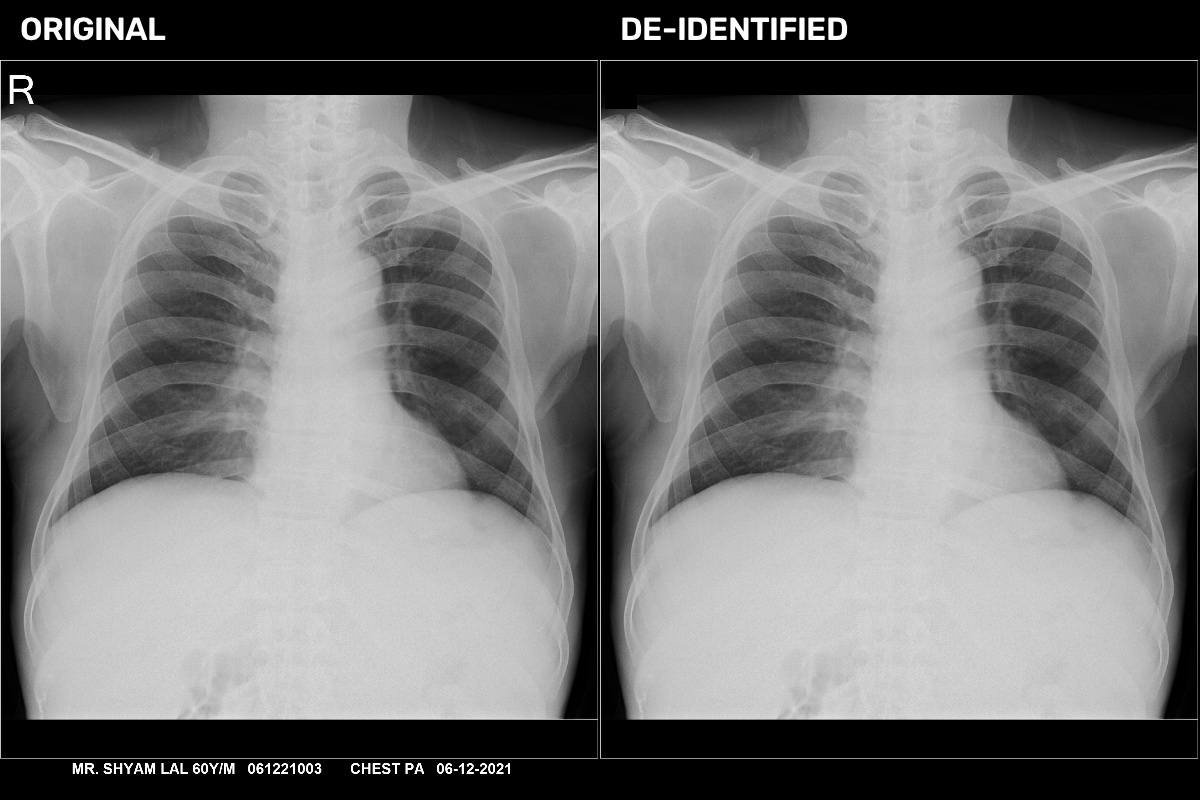
\includegraphics[width=0.98\linewidth]{results/deidentified/client2_01_comparison.jpg}
\caption{Representative chest X-ray radiograph before and after the OCR-based de-identification pipeline. Visible patient demographics and hospital acquisition text are detected and masked while preserving the anatomical thoracic region.}
\label{fig:deidentification}
\end{figure}

Following de-identification, input images undergo the standardized preprocessing pipeline. As illustrated in Figure~\ref{fig:preprocessing}, applying Contrast Limited Adaptive Histogram Equalization (CLAHE) substantially enhances local contrast across the thoracic cavity, amplifying faint parenchymal densities, interstitial markings, and pleural contours. The images are subsequently resized to $224 \times 224$ and standardized using ImageNet normalization parameters prior to model ingestion.

\begin{figure}[t]
\centering
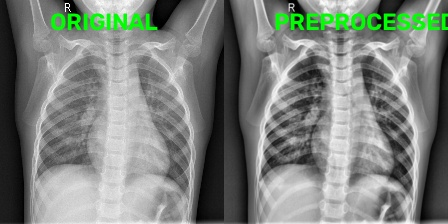
\includegraphics[width=0.98\linewidth]{results/preprocessing/client1_preprocessing_comparison.jpg}
\caption{Representative output of the image preprocessing stage comparing the original radiograph (left) with the CLAHE contrast-enhanced and normalized input tensor (right).}
\label{fig:preprocessing}
\end{figure}

\subsection{Global Model Convergence Across Rounds}
Table~\ref{tab:global_performance} and Figure~\ref{fig:performance_rounds} illustrate the pooled evaluation metrics across the three federated rounds. 

\begin{table}[h]
\centering
\caption{Pooled Global Model Test Performance Across Communication Rounds}
\label{tab:global_performance}
\begin{tabular}{ccccc}
\toprule
\textbf{Round} & \textbf{Accuracy (\%)} & \textbf{Precision (\%)} & \textbf{Recall (\%)} & \textbf{F1-Score (\%)} \\
\midrule
Round 1 & 80.59 & 81.25 & \textbf{85.81} & \textbf{83.47} \\
Round 2 & 80.03 & 83.12 & 81.60 & 82.35 \\
Round 3 & \textbf{81.40} & \textbf{86.25} & 80.20 & 83.11 \\
\bottomrule
\end{tabular}
\end{table}

\begin{figure}[t]
\centering
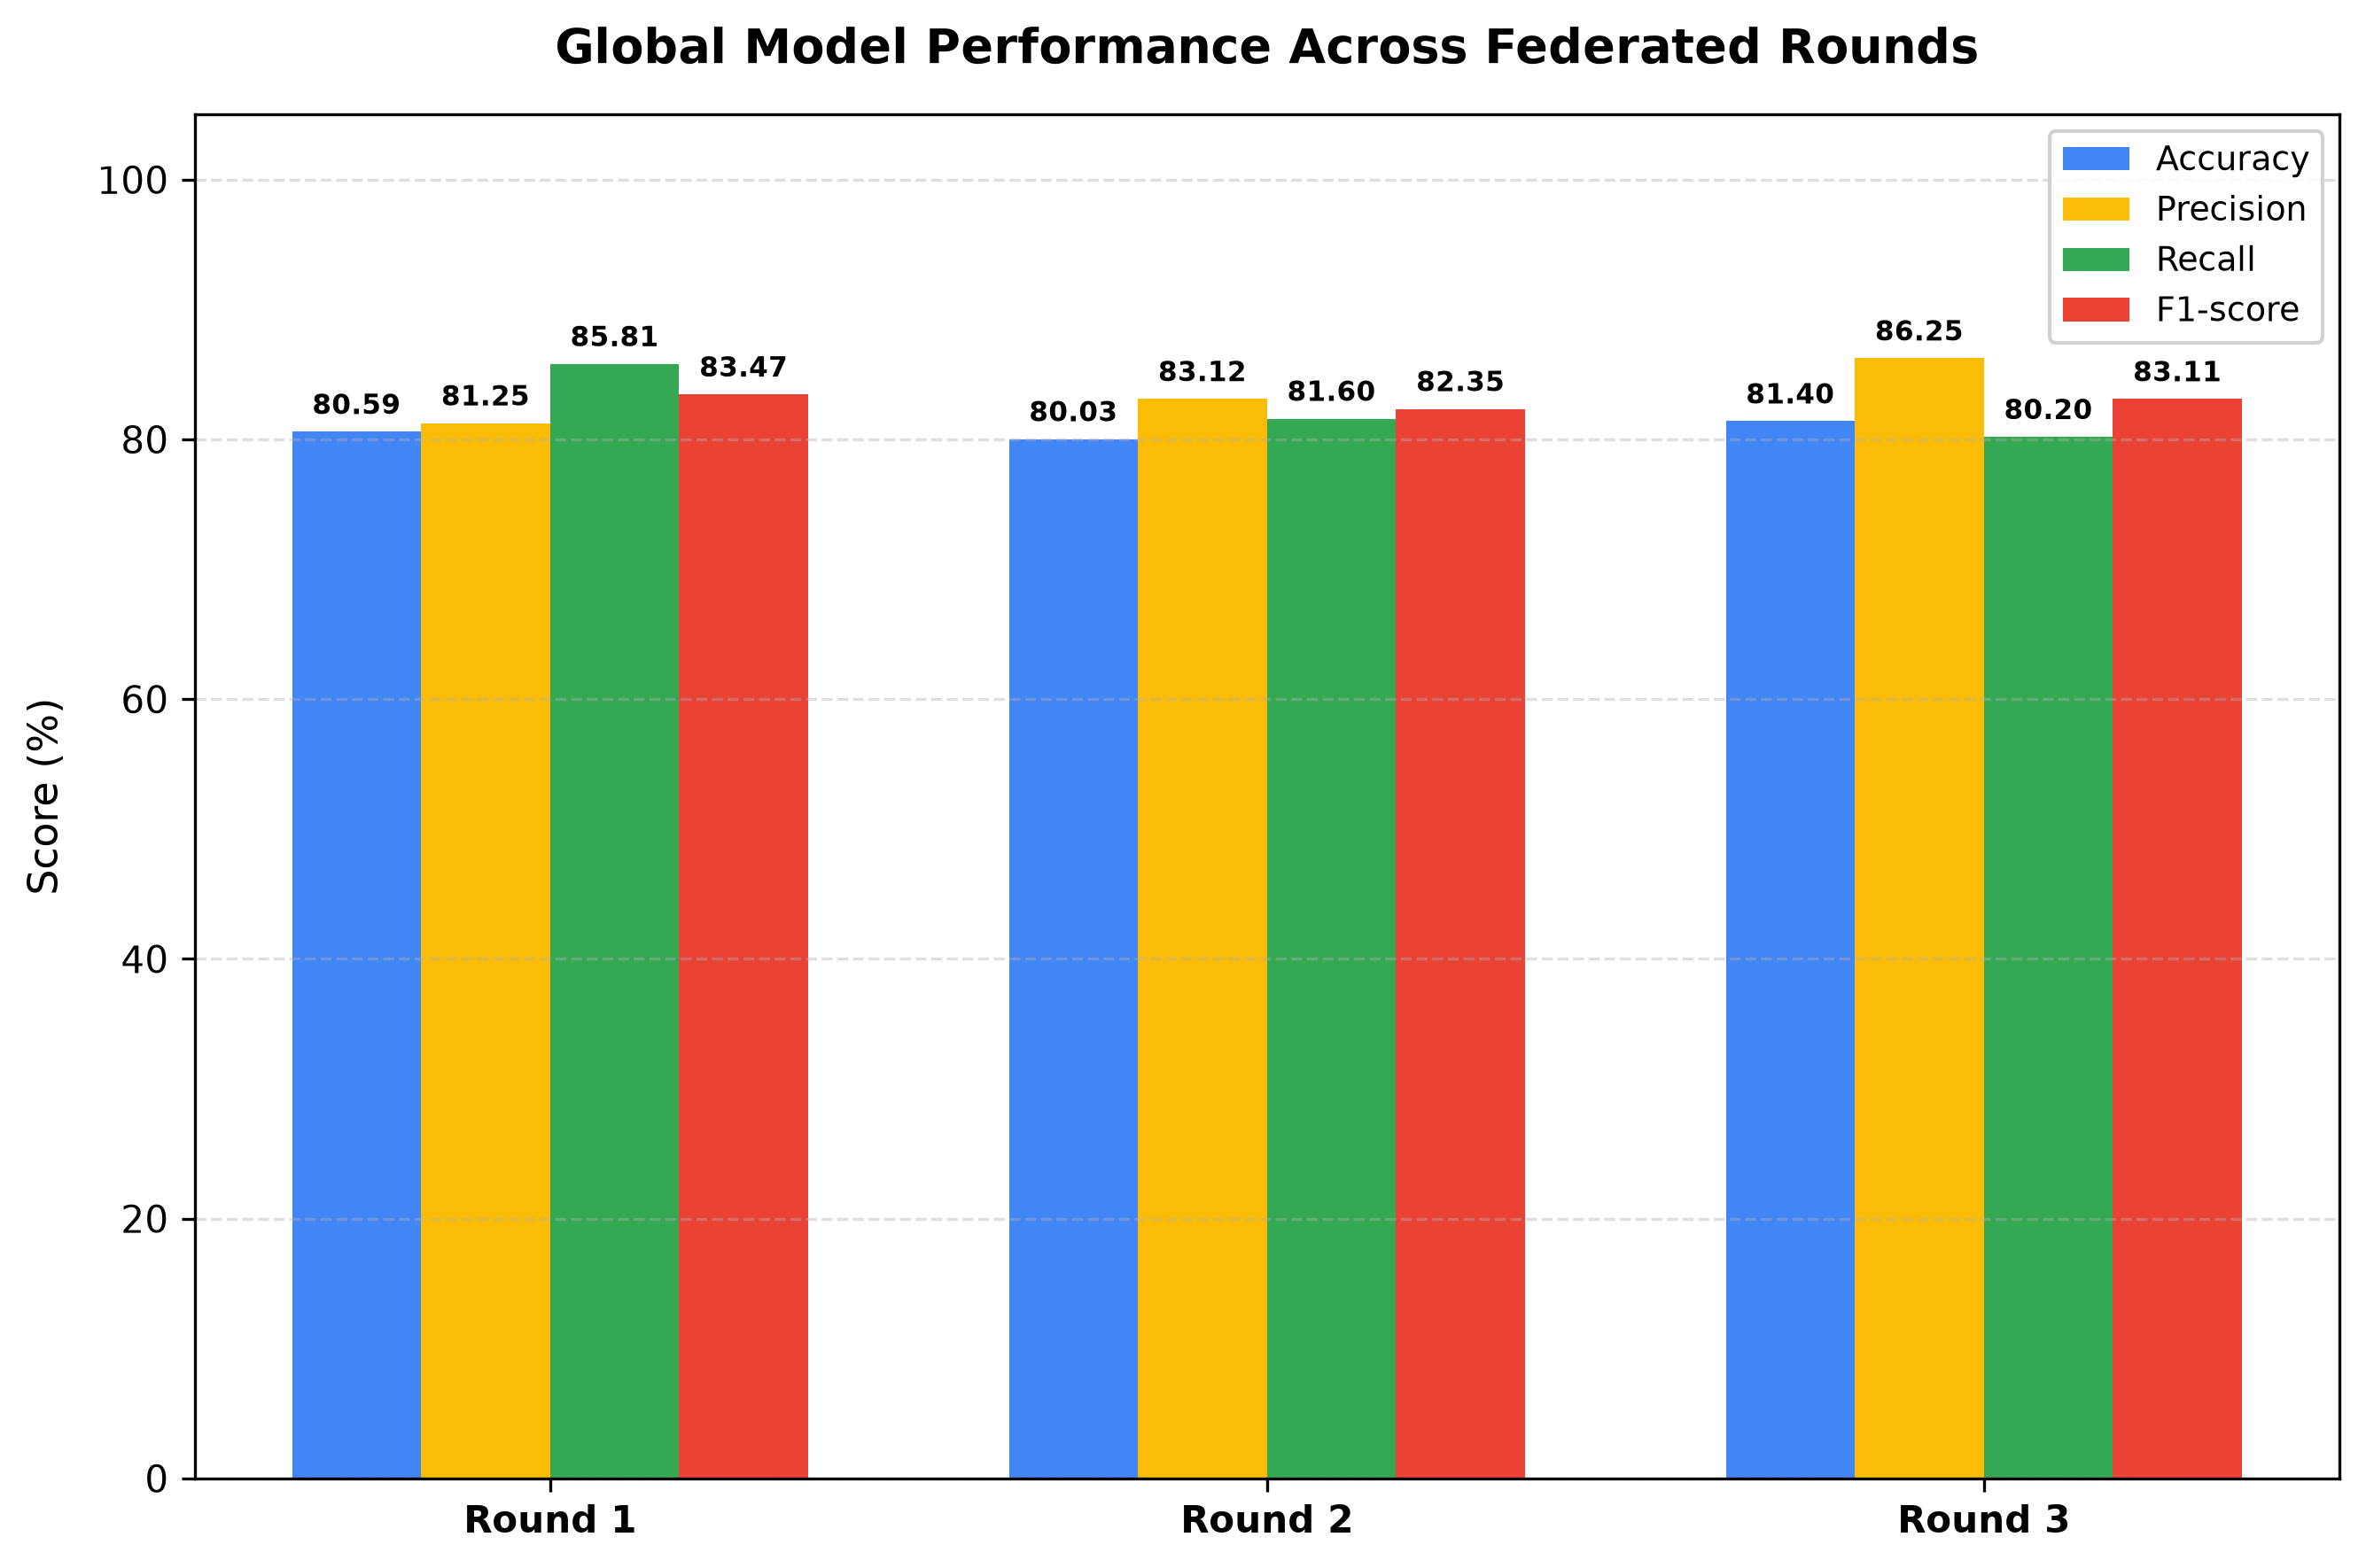
\includegraphics[width=0.95\linewidth]{results/visualizations/fig4_performance_rounds.png}
\caption{Accuracy, precision, recall, and F1-score of the global federated model across three communication rounds.}
\label{fig:performance_rounds}
\end{figure}

The global model achieves its highest overall accuracy (81.40\%) and precision (86.25\%) at Round 3. Conversely, Round 1 exhibited superior sensitivity (85.81\%) and F1-score (83.47\%). In parallel, local validation monitoring recorded progressive accuracy improvements from 84.77\% in Round 1, to 87.89\% in Round 2, and 90.04\% in Round 3, corroborating the stability provided by the FedProx proximal constraint.

\subsection{Pooled Confusion Matrix Analysis}
The cumulative test confusion matrix for Round 3 across all 1,247 held-out radiographs (535 Normal, 712 Pneumonia) is shown in Figure~\ref{fig:confusion_matrix}:
\begin{equation}
C = \begin{bmatrix} 444 & 91 \\ 141 & 571 \end{bmatrix}
\end{equation}
The model correctly identifies 444 normal lungs (specificity = 83.00\%) and 571 pneumonia cases (sensitivity = 80.20\%). The 141 false negatives represent patients with early-stage or faint bronchopneumonic infiltrates misclassified as normal, demonstrating an area where federated consensus requires further sensitivity weighting.

\begin{figure}[t]
\centering
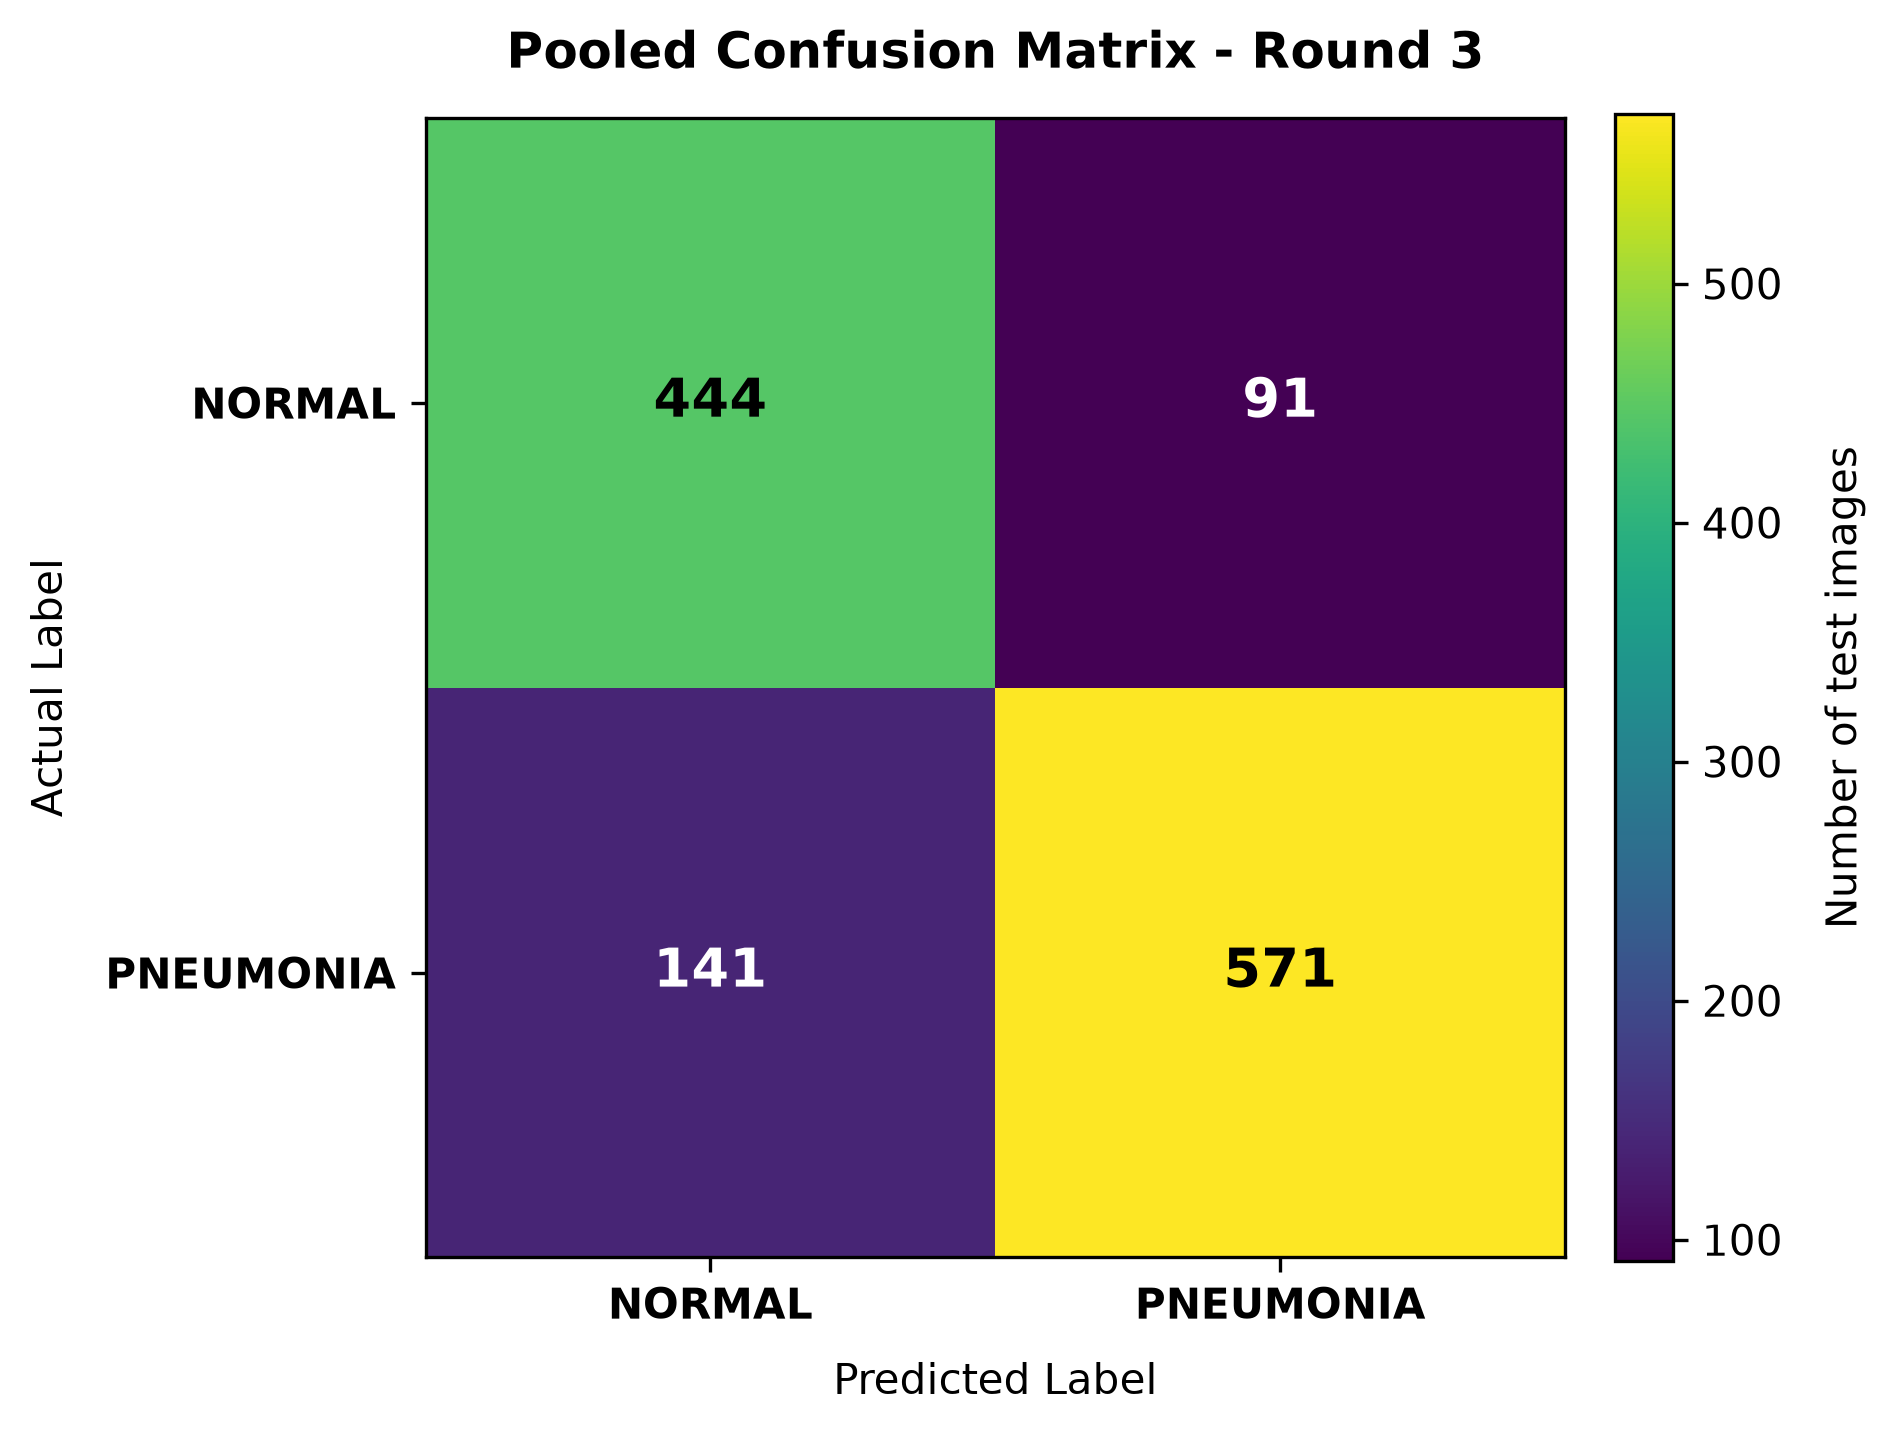
\includegraphics[width=0.85\linewidth]{results/visualizations/fig7_confusion_matrix.png}
\caption{Pooled confusion matrix of the global model after Round 3 on 1,247 combined test images ($C_{11}=444$, $C_{12}=91$, $C_{21}=141$, $C_{22}=571$).}
\label{fig:confusion_matrix}
\end{figure}

\subsection{Client-Wise Discrepancy Analysis}
Evaluating model updates on individual institutional cohorts illuminates the impact of non-IID distributions, as tabulated in Table~\ref{tab:client_performance} and depicted in Figure~\ref{fig:client_performance}.

\begin{table}[h]
\centering
\caption{Client-Wise Classification Performance in Round 3}
\label{tab:client_performance}
\begin{tabular}{lcccc}
\toprule
\textbf{Client Site} & \textbf{Accuracy} & \textbf{Precision} & \textbf{Recall} & \textbf{F1-Score} \\
\midrule
Client 1 (Kaggle)     & 85.42\% & 81.21\%  & 99.74\% & 89.53\% \\
Client 2 (Chittagong) & 45.45\% & 100.00\% & 9.09\%  & 16.67\% \\
Client 3 (Bhopal)     & 84.21\% & 99.44\%  & 68.75\% & 81.29\% \\
\bottomrule
\end{tabular}
\end{table}

\begin{figure}[t]
\centering
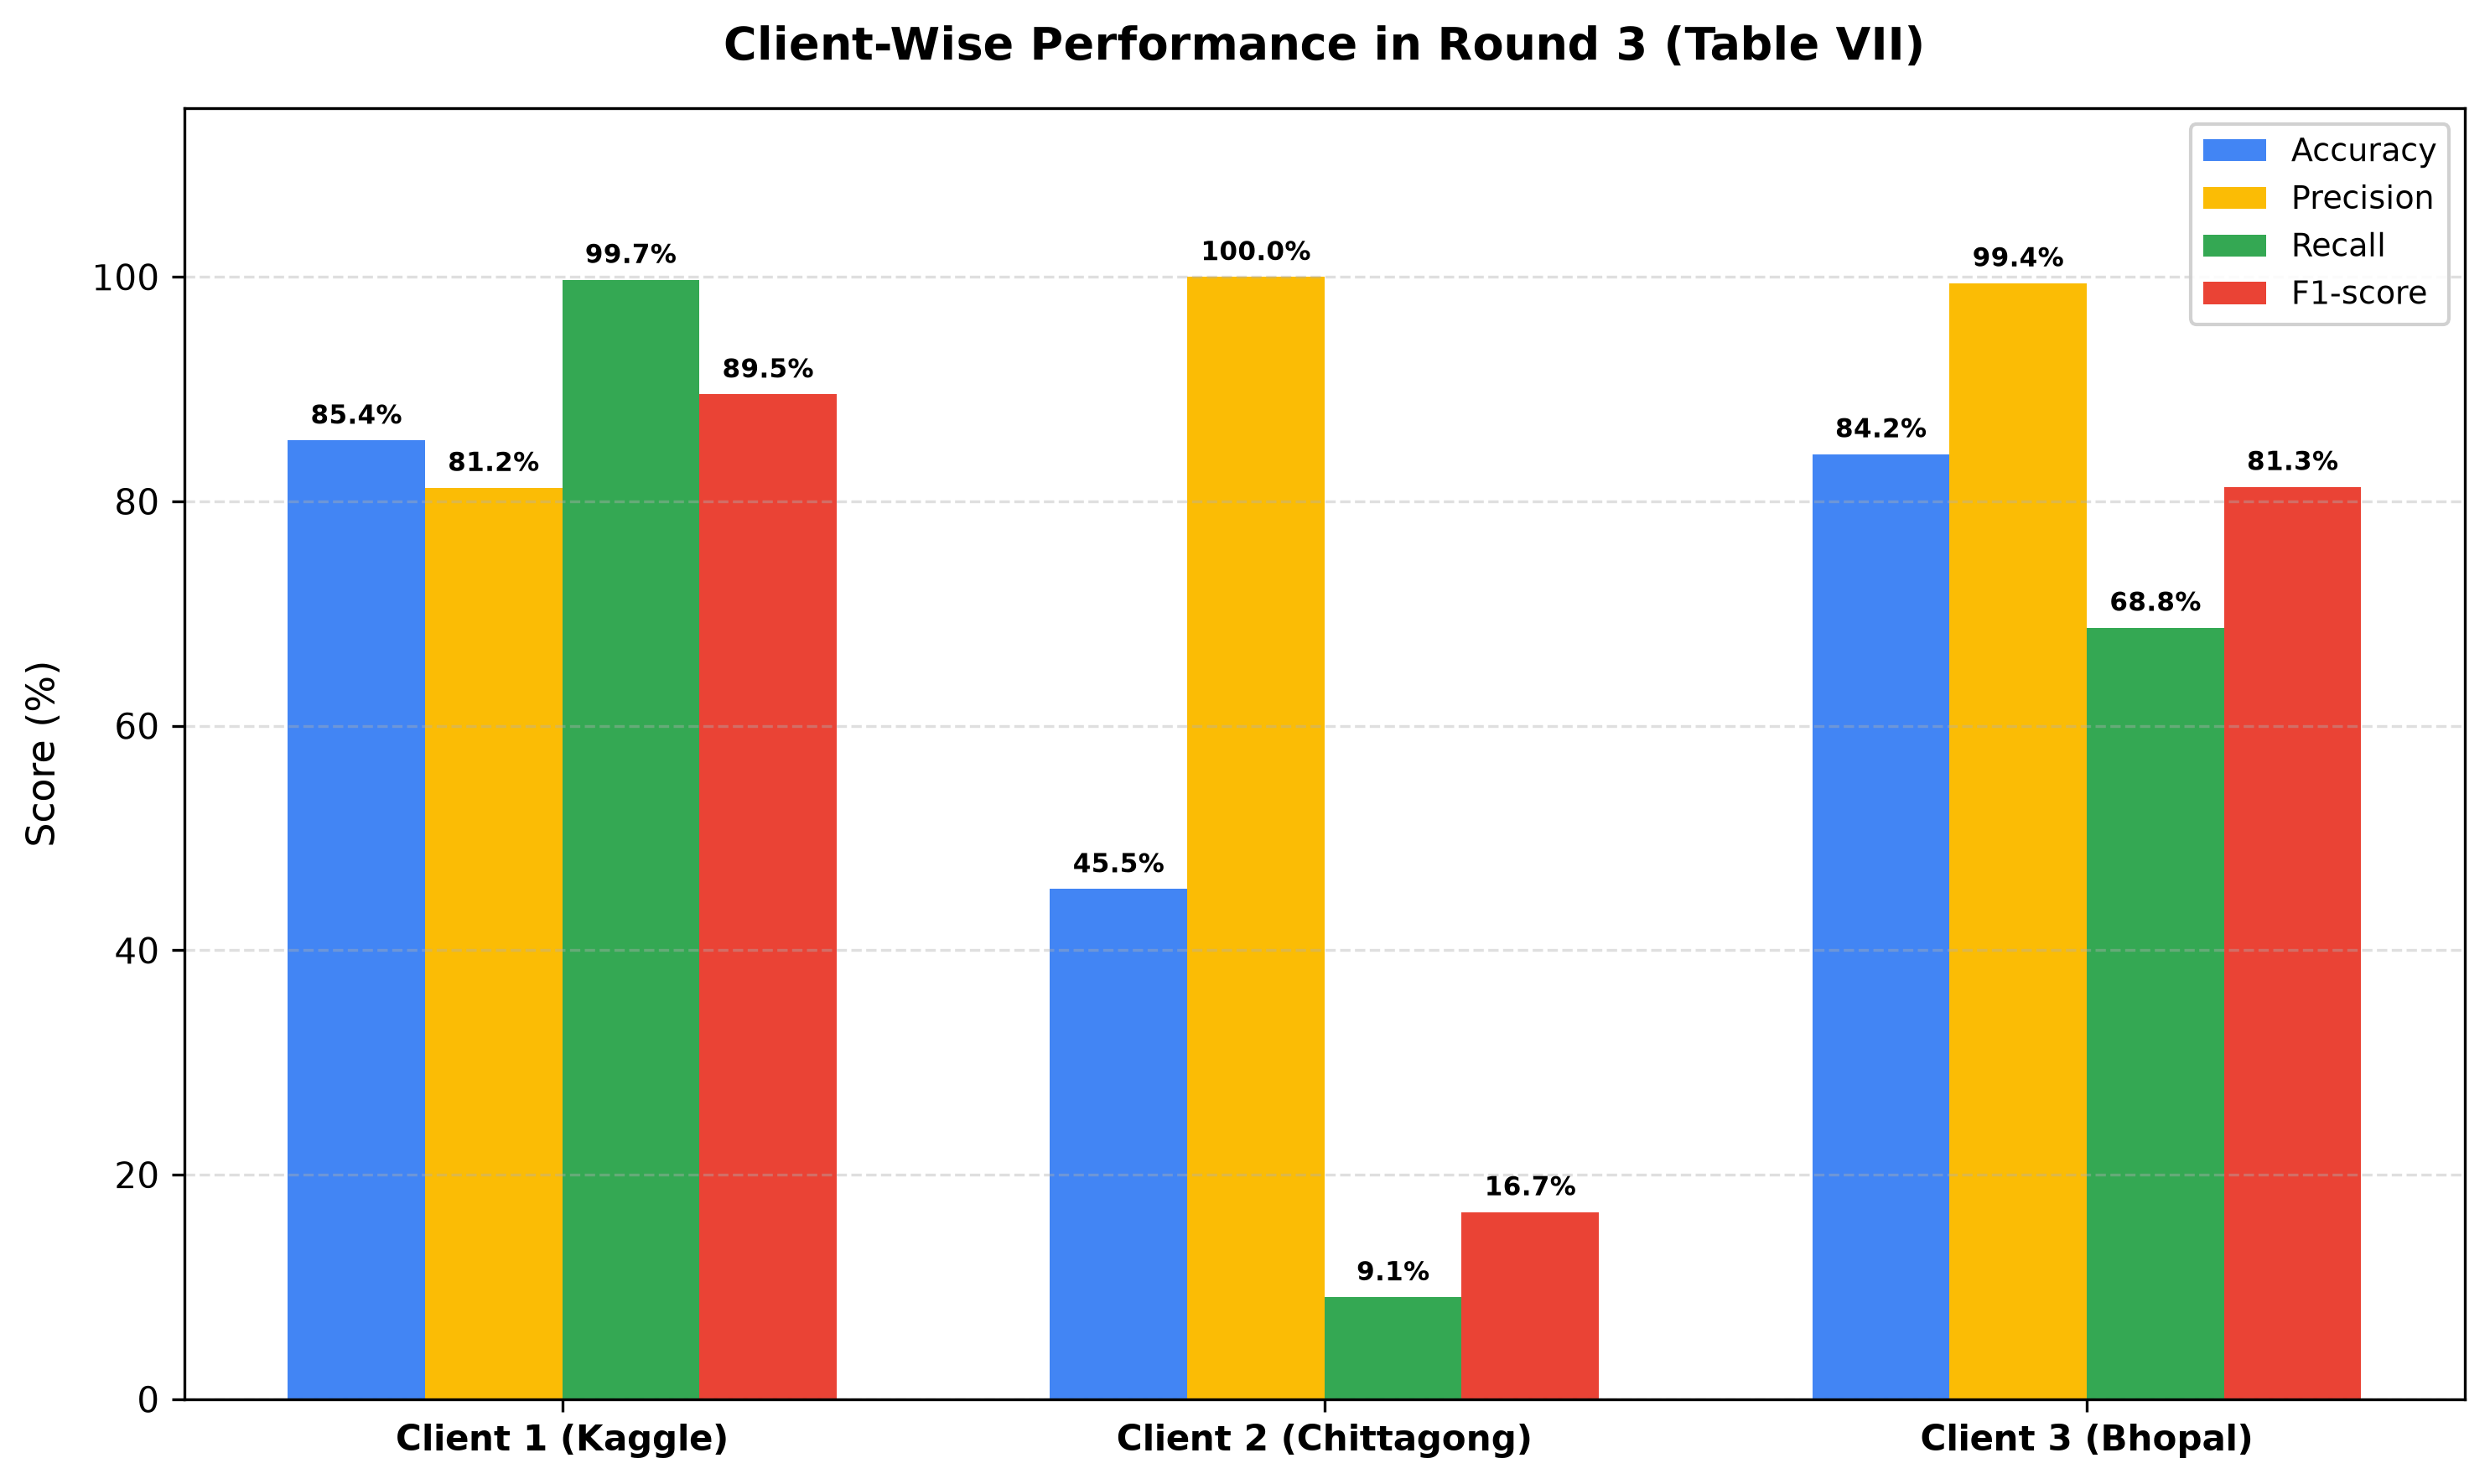
\includegraphics[width=0.95\linewidth]{results/visualizations/client_performance_round3.png}
\caption{Disaggregated client-wise diagnostic performance across the three participating institutions in Round 3.}
\label{fig:client_performance}
\end{figure}

The disaggregated breakdown reveals notable clinical dynamics:
\begin{itemize}
    \item \textbf{Client 1:} Exhibits exceptional recall (99.74\%) and F1-score (89.53\%), effectively catching nearly all pneumonia cases.
    \item \textbf{Client 2:} Displays a severe drop in recall (9.09\%) despite 100\% precision. The smaller cohort size (320 training images) combined with differing radiograph contrast caused the global model to adopt an ultra-conservative decision threshold for this domain.
    \item \textbf{Client 3:} Shows high precision (99.44\%) and balanced accuracy (84.21\%), with moderate recall (68.75\%).
\end{itemize}
These findings demonstrate an essential insight for clinical federated learning: \textit{aggregate pooled accuracy can easily obscure acute underperformance at specific participating sites.}

\subsection{Latent Feature Space Representation}
To inspect the internal feature representations learned by the federated backbone, 2048-dimensional embeddings extracted from \texttt{layer4} across held-out client test samples were mapped to 2D projections via t-SNE and PCA, as shown in Figure~\ref{fig:latent_space}.

\begin{figure}[t]
\centering
\begin{subfigure}[b]{0.48\linewidth}
    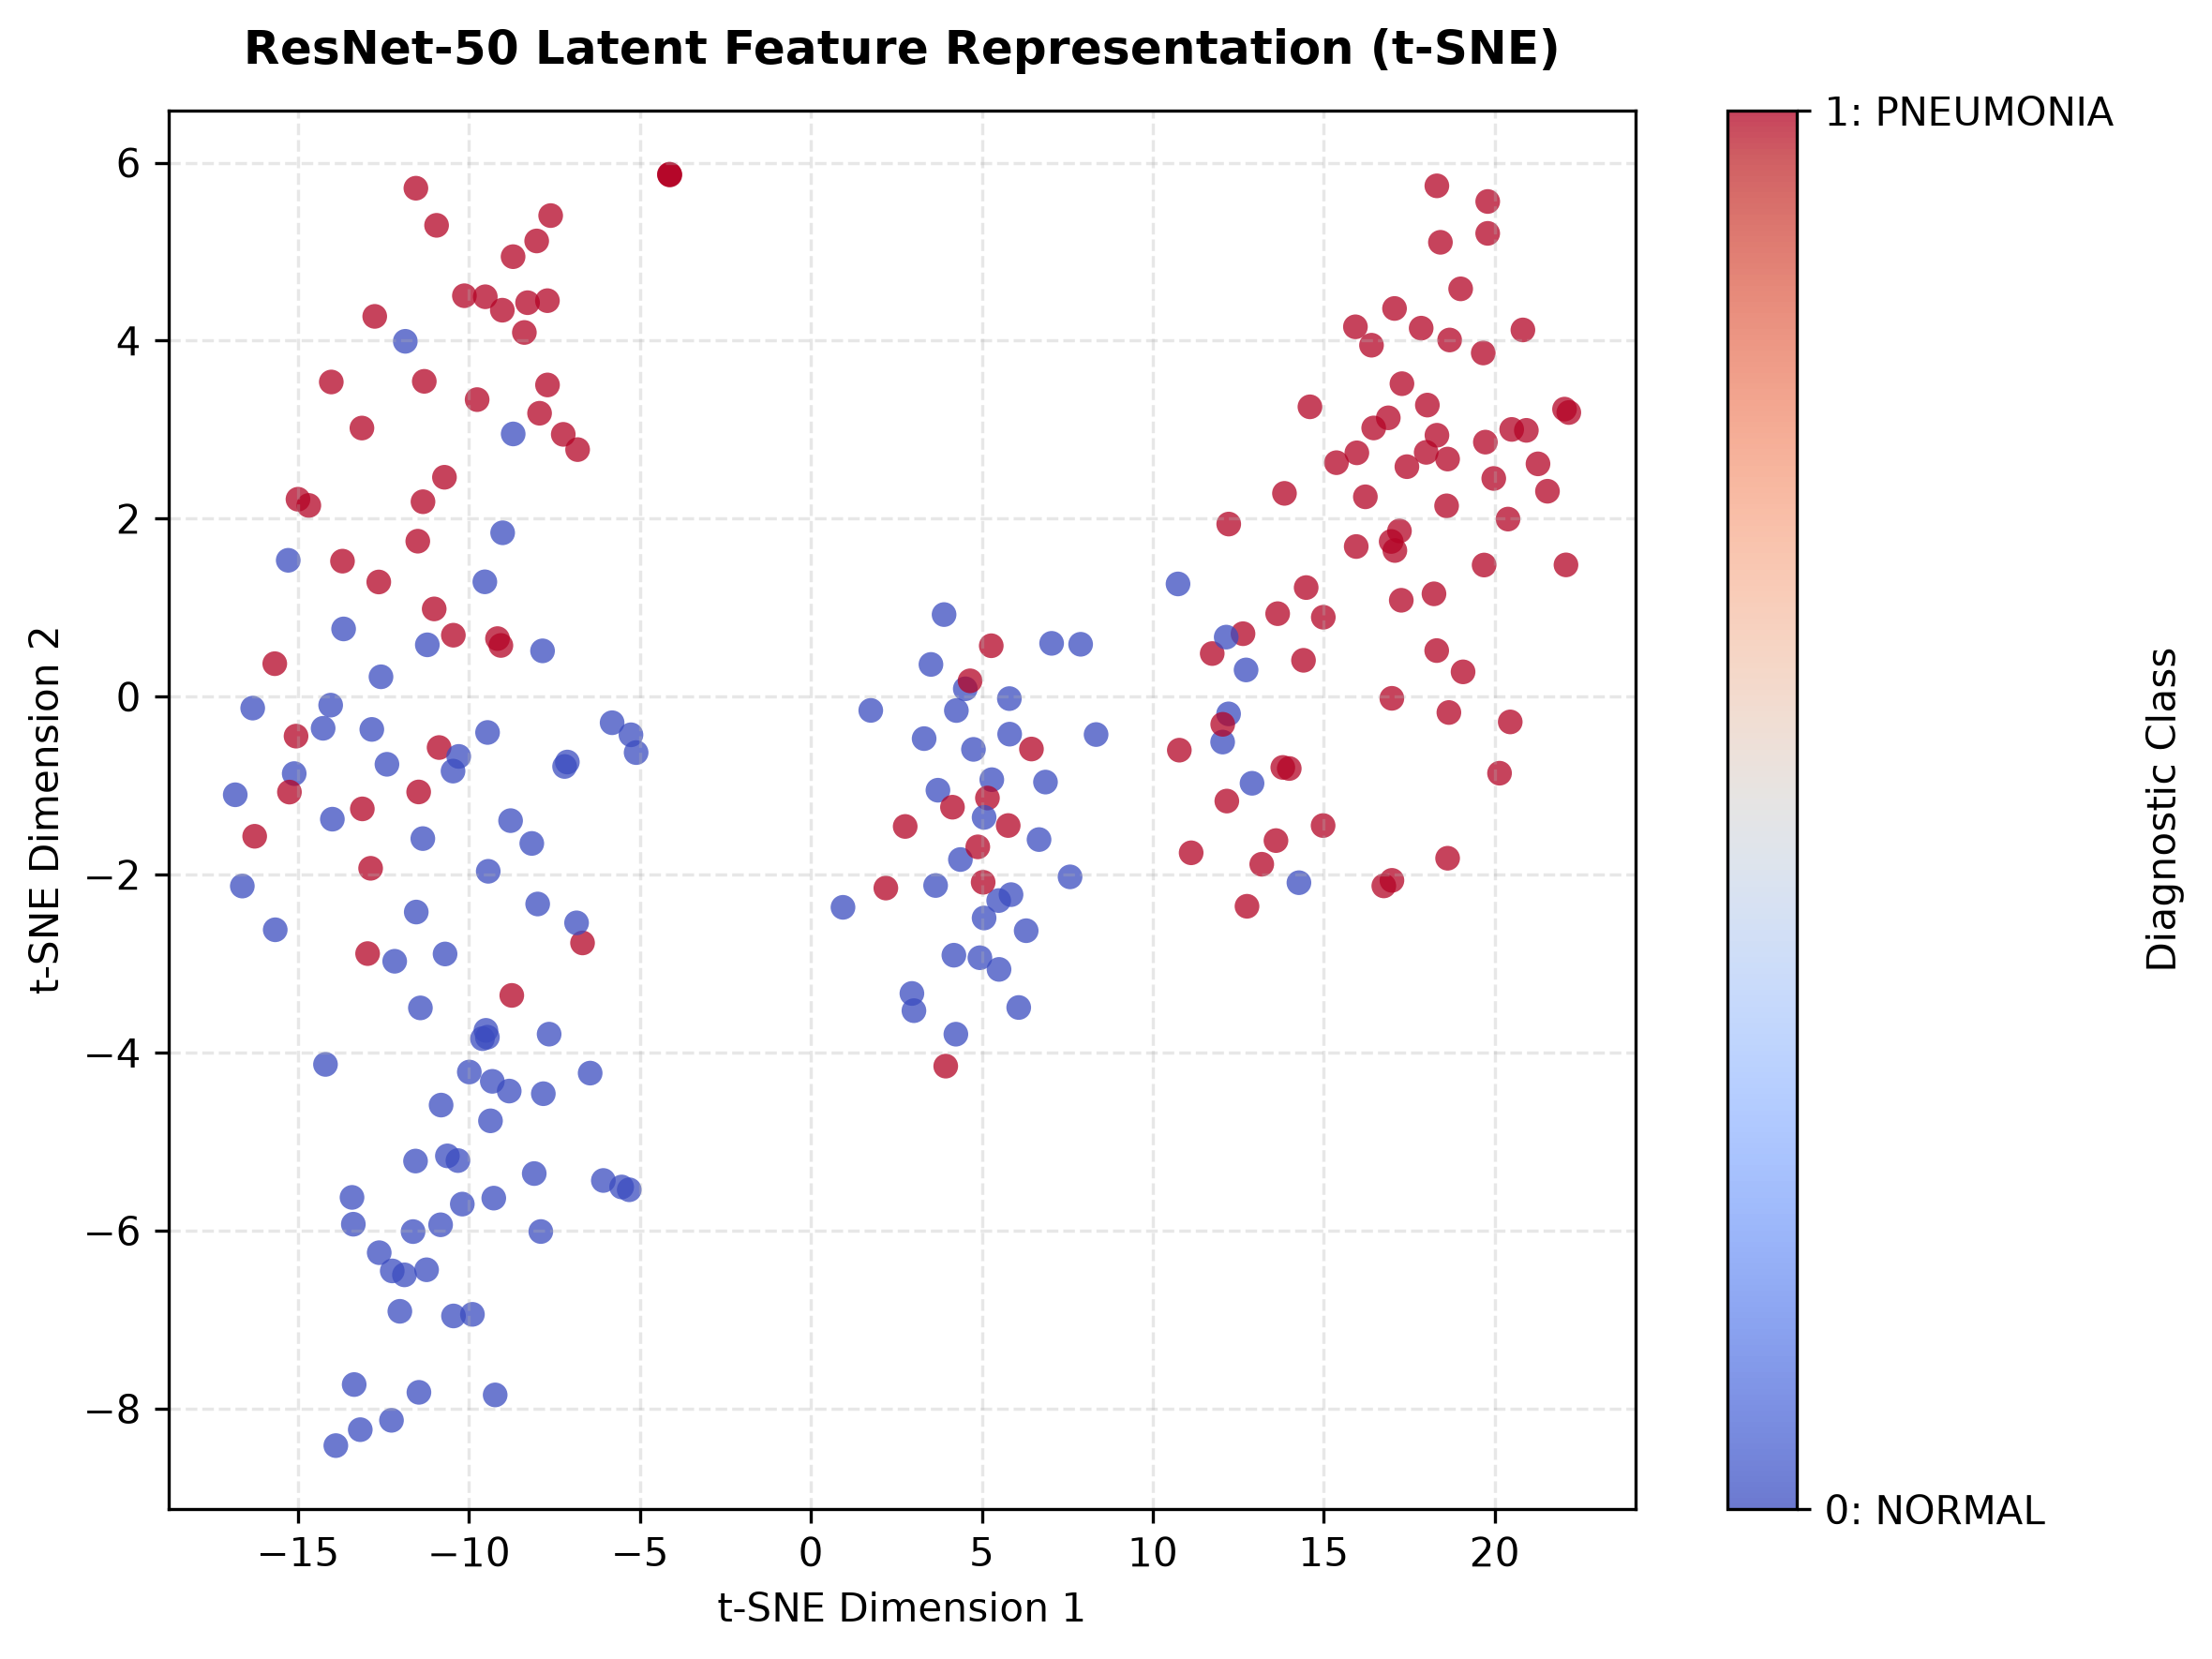
\includegraphics[width=\linewidth]{results/visualizations/resnet50_latent_tsne.png}
    \caption{t-SNE Projection}
\end{subfigure}
\hfill
\begin{subfigure}[b]{0.48\linewidth}
    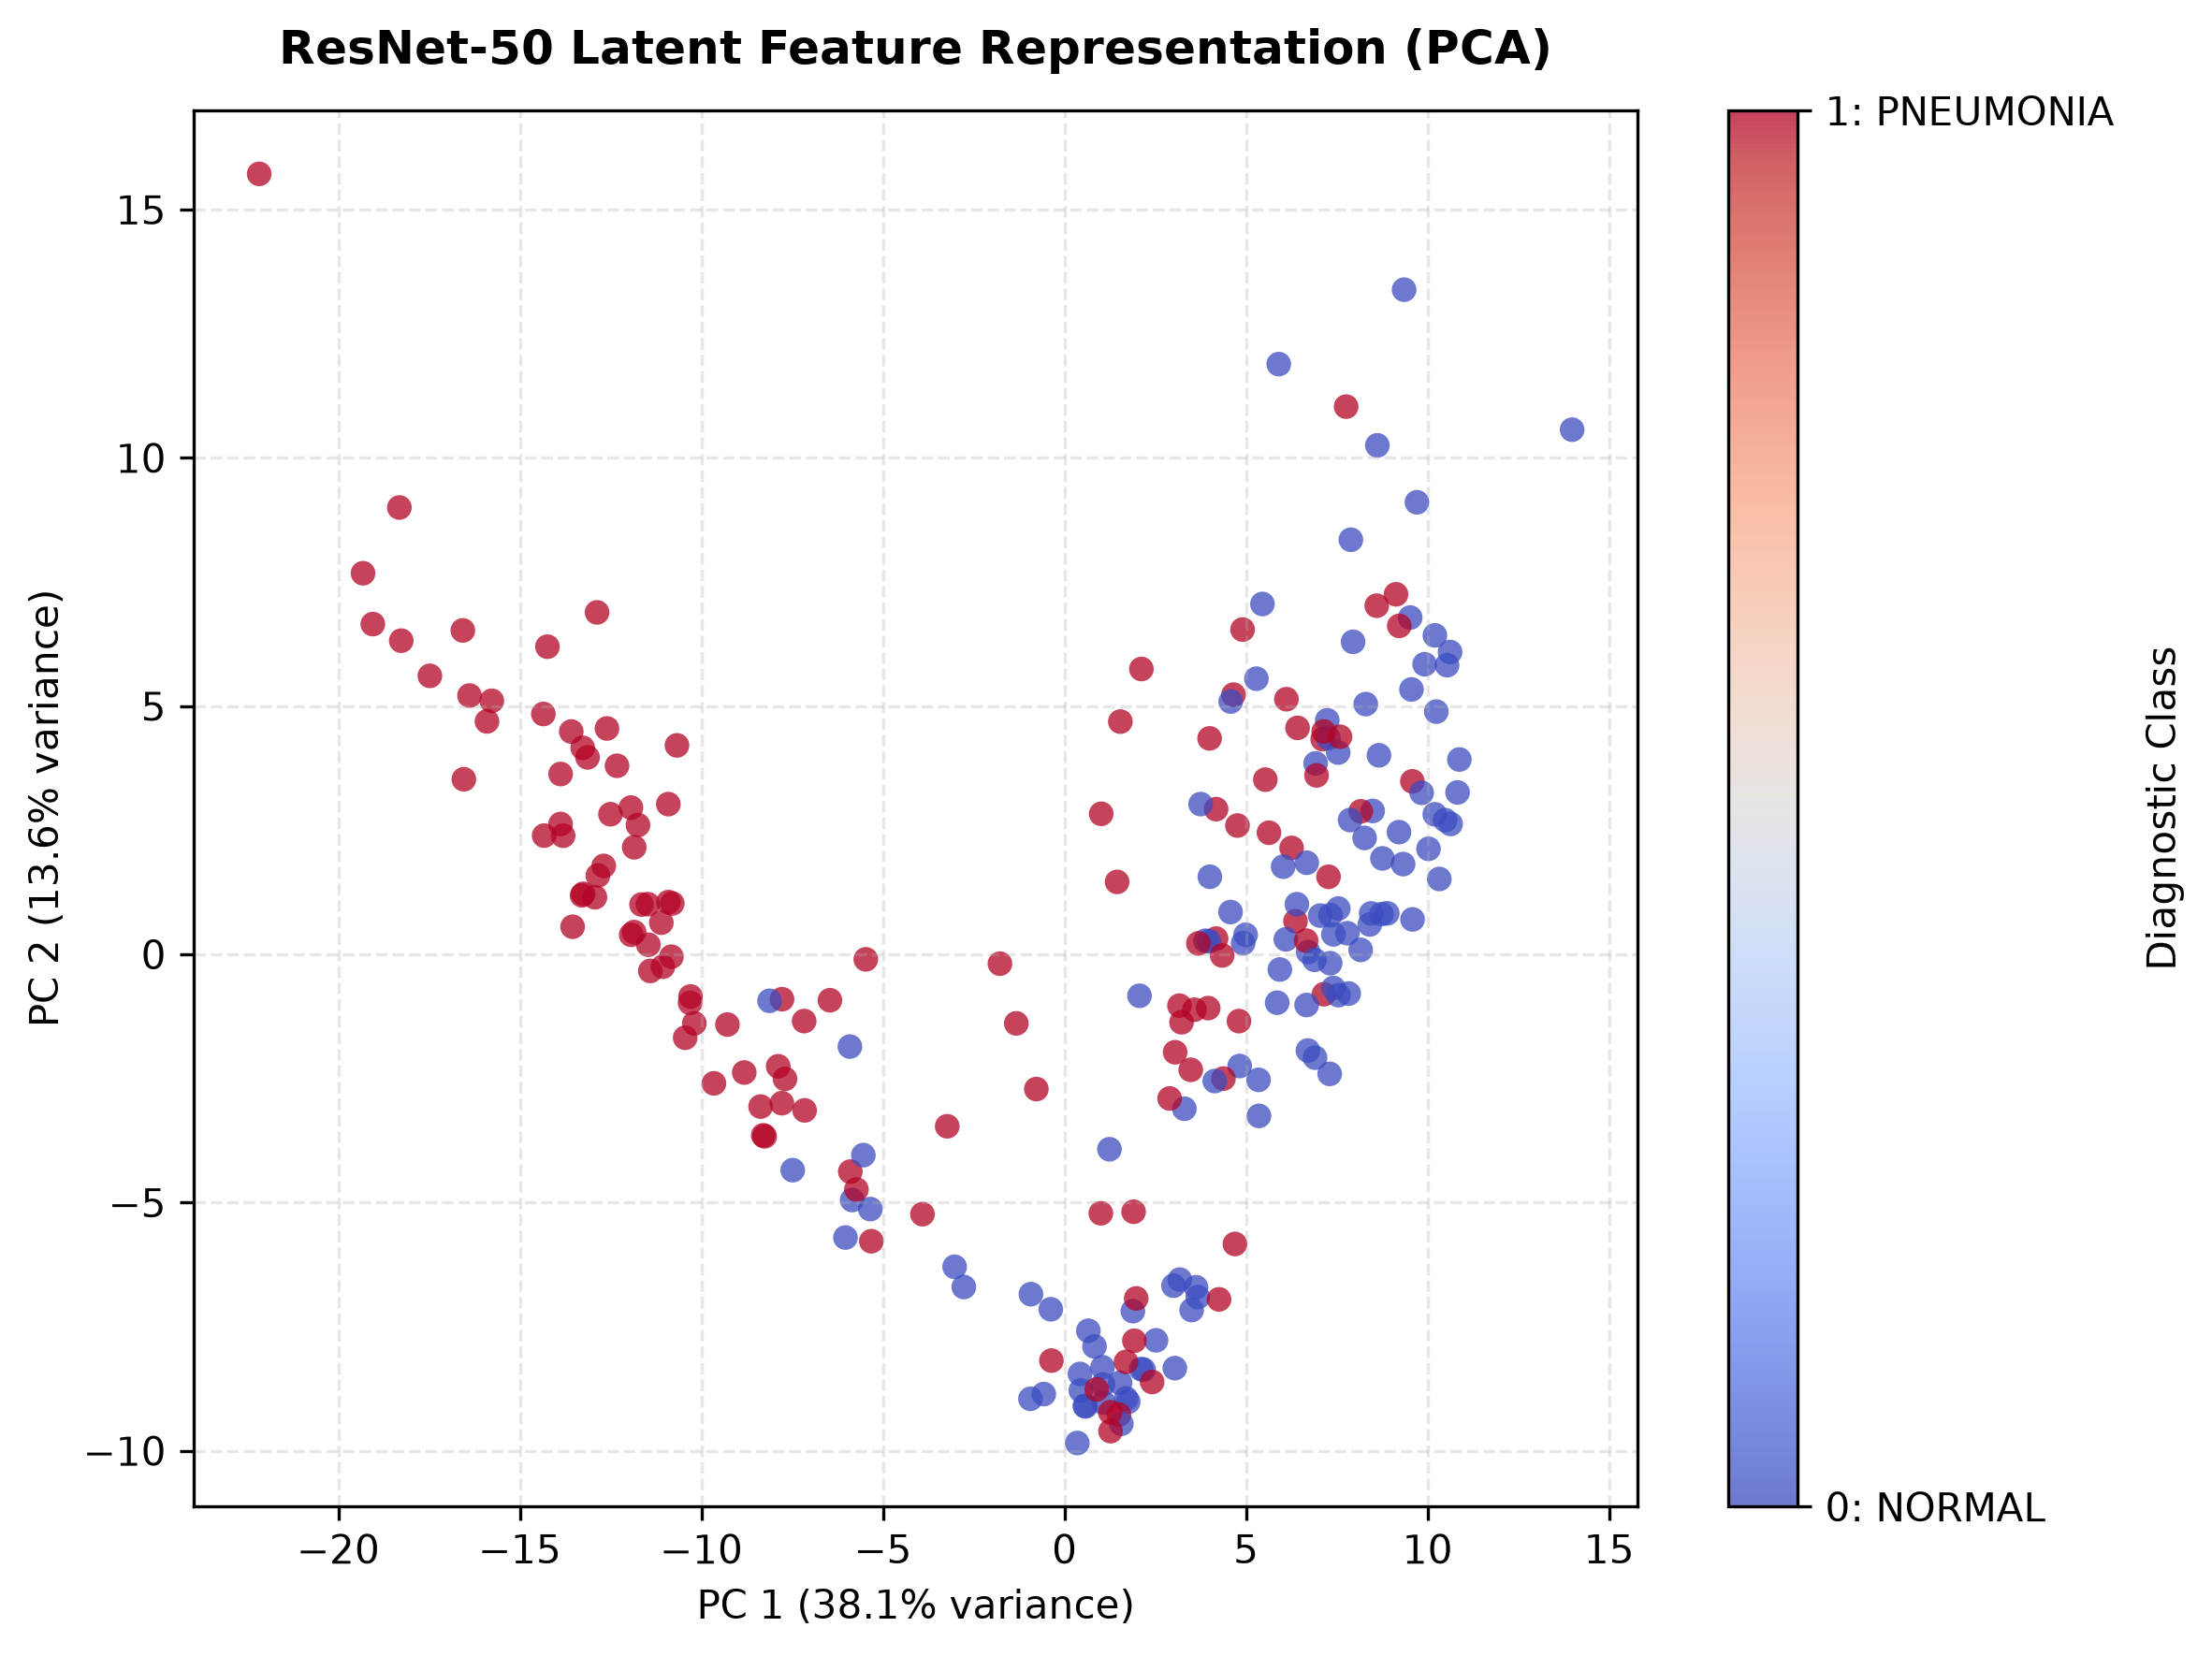
\includegraphics[width=\linewidth]{results/visualizations/resnet50_latent_pca.png}
    \caption{PCA Projection}
\end{subfigure}
\caption{2D latent space projections of 2048-dimensional ResNet-50 feature representations extracted from test radiographs, demonstrating class clustering between NORMAL (blue) and PNEUMONIA (red).}
\label{fig:latent_space}
\end{figure}

The latent space visualization demonstrates distinct clustering between NORMAL and PNEUMONIA representations. The boundary overlap aligns with low-confidence cases where radiographic features exhibit mild or ambiguous infiltrates.

\subsection{Explainability via Grad-CAM}
Grad-CAM heatmaps verify that the global federated network bases its diagnostic predictions on pulmonary regions rather than spurious edge artifacts.

\begin{figure}[t]
\centering
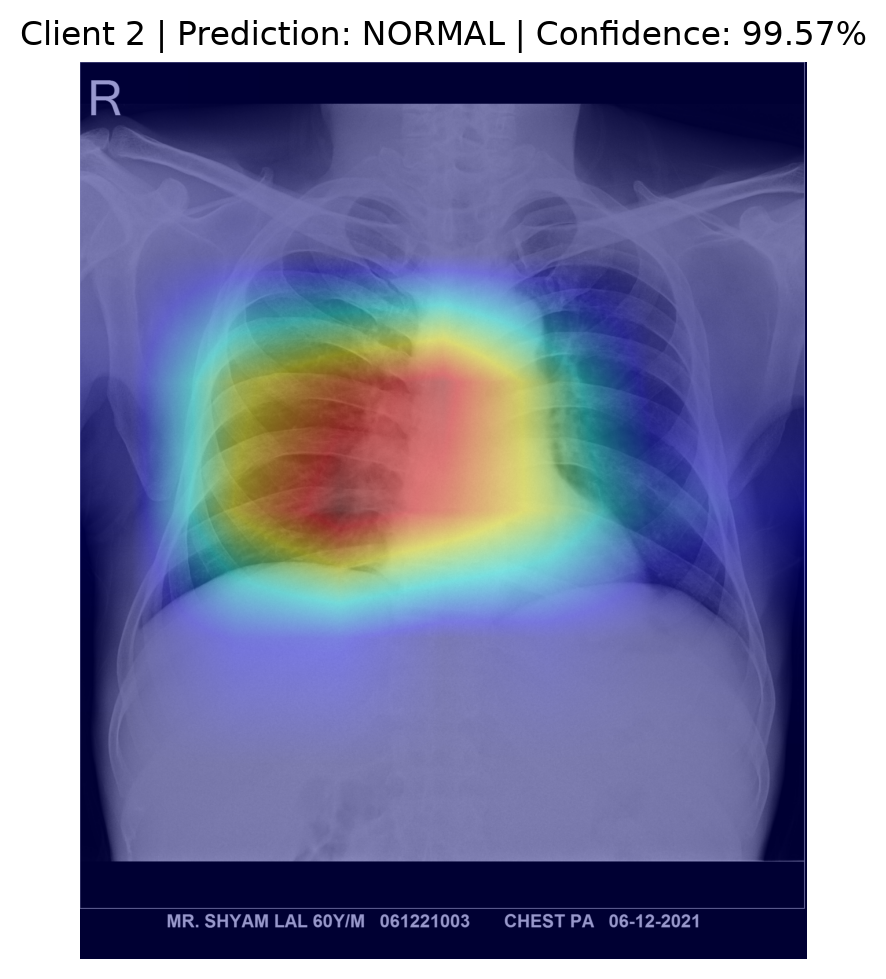
\includegraphics[width=0.85\linewidth]{results/visualizations/client2_normal_01_gradcam.png}
\caption{Representative visual explainability output generated by the federated ResNet-50 model via Grad-CAM, indicating localized lung parenchymal attention.}
\label{fig:gradcam}
\end{figure}

As shown in Figure~\ref{fig:gradcam}, the network focuses attention over lower lobe lung fields rather than peripheral borders or masked metadata areas, confirming the efficacy of the automated de-identification and CLAHE pipeline.

\section{Conclusion and Future Work}
This study presented a privacy-preserving federated diagnostic framework for pneumonia detection across heterogeneous chest X-ray datasets. Integrating ResNet-50 transfer learning, proximal FedProx regularization, and TLS mutual encryption enabled collaborative model training without raw data centralization. Across 6,363 radiographs from three multi-institutional centers, the round-3 global model achieved a pooled accuracy of 81.40\%, precision of 86.25\%, and F1-score of 83.11\%.

Importantly, our disaggregated analysis exposed substantial client-level performance variance (e.g., Client 2 recall of 9.09\%), proving that global metrics alone are insufficient to guarantee cross-site reliability. Grad-CAM visual heatmaps and t-SNE latent representations confirmed that the architecture concentrates on relevant pulmonary pathology. Future extensions will focus on personalized federated algorithms (e.g., FedPer, pFedMe), adaptive threshold calibration per site, and integration of formal differential privacy (DP-SGD) with cryptographic secure aggregation.

\begin{thebibliography}{00}

\bibitem{wang2017chestxray8}
X.~Wang, Y.~Peng, L.~Lu, Z.~Lu, M.~Bagheri, and R.~M.~Summers, ``ChestX-ray8: Hospital-scale chest X-ray database and benchmarks on weakly-supervised classification and localization of common thorax diseases,'' in \textit{Proc. IEEE CVPR}, 2017, pp. 2097--2106.

\bibitem{rajpurkar2017chexnet}
P.~Rajpurkar, J.~Irvin, K.~Zhu, B.~Yang, H.~Mehta, T.~Duan, D.~Ding, A.~Bagul, R.~L.~Ball, C.~Langlotz, K.~Shpanskaya, M.~P.~Lungren, and A.~Y.~Ng, ``CheXNet: Radiologist-level pneumonia detection on chest X-rays with deep learning,'' \textit{arXiv:1711.05225}, 2017.

\bibitem{irvin2019chexpert}
J.~Irvin, P.~Rajpurkar, M.~Ko, Y.~Yu, S.~Ciurea-Ilcus, C.~Chute, H.~Marklund, B.~Haghgoo, R.~L.~Ball, K.~Shpanskaya, J.~Seekins, D.~A.~Mong, S.~S.~Halabi, J.~K.~Sandberg, R.~Jones, D.~B.~Larson, C.~P.~Langlotz, B.~N.~Patel, M.~P.~Lungren, and A.~Y.~Ng, ``CheXpert: A large chest radiograph dataset with uncertainty labels and expert comparison,'' in \textit{Proc. AAAI}, vol.~33, 2019, pp. 590--597.

\bibitem{he2016deep}
K.~He, X.~Zhang, S.~Ren, and J.~Sun, ``Deep residual learning for image recognition,'' in \textit{Proc. IEEE CVPR}, 2016, pp. 770--778.

\bibitem{mcmahan2017communication}
B.~McMahan, E.~Moore, D.~Ramage, S.~Hampson, and B.~A.~y~Arcas, ``Communication-efficient learning of deep networks from decentralized data,'' in \textit{Proc. AISTATS}, vol.~54, 2017, pp. 1273--1282.

\bibitem{kairouz2021advances}
P.~Kairouz \textit{et al.}, ``Advances and open problems in federated learning,'' \textit{Foundations and Trends in Machine Learning}, vol.~14, nos.~1--2, pp. 1--210, 2021.

\bibitem{li2020federated}
T.~Li, A.~K.~Sahu, M.~Zaheer, M.~Sanjabi, A.~Talwalkar, and V.~Smith, ``Federated optimization in heterogeneous networks,'' in \textit{Proc. MLSys}, vol.~2, 2020, pp. 429--450.

\bibitem{rieke2020future}
N.~Rieke \textit{et al.}, ``The future of digital health with federated learning,'' \textit{npj Digital Medicine}, vol.~3, art.~119, 2020.

\bibitem{sheller2019multi}
M.~J.~Sheller, G.~A.~Reina, B.~Edwards, J.~Martin, and S.~Bakas, ``Multi-institutional deep learning modeling without sharing patient data: A feasibility study on brain tumor segmentation,'' in \textit{Brainlesion}, 2019, pp. 92--104.

\bibitem{sheller2020federated}
M.~J.~Sheller \textit{et al.}, ``Federated learning in medicine: Facilitating multi-institutional collaborations without sharing patient data,'' \textit{Scientific Reports}, vol.~10, art.~12598, 2020.

\bibitem{kaissis2020secure}
G.~A.~Kaissis, M.~R.~Makowski, D.~R\"uckert, and R.~F.~Braren, ``Secure, privacy-preserving and federated machine learning in medical imaging,'' \textit{Nature Machine Intelligence}, vol.~2, pp. 305--311, 2020.

\bibitem{li2024federated}
W.~Li \textit{et al.}, ``Federated learning for medical image analysis: A survey,'' \textit{Medical Image Analysis}, 2024.

\bibitem{selvaraju2017gradcam}
R.~R.~Selvaraju, M.~Cogswell, A.~Das, R.~Vedantam, D.~Parikh, and D.~Batra, ``Grad-CAM: Visual explanations from deep networks via gradient-based localization,'' in \textit{Proc. IEEE ICCV}, 2017, pp. 618--626.

\bibitem{zhu2019deep}
L.~Zhu, Z.~Liu, and S.~Han, ``Deep leakage from gradients,'' in \textit{Advances in Neural Information Processing Systems}, vol.~32, 2019.

\bibitem{hipaa1996}
Health Insurance Portability and Accountability Act of 1996, Pub. L. No. 104-191, 110 Stat. 1936, 1996.

\bibitem{hhs2003}
U.S. Department of Health and Human Services, ``Security standards for the protection of electronic protected health information,'' 45 C.F.R. Parts 160 and 164, 2003.

\bibitem{gdpr2016}
European Parliament and Council of the European Union, ``Regulation (EU) 2016/679 (General Data Protection Regulation),'' \textit{Official Journal of the European Union}, 2016.

\bibitem{zhou2026federated}
Z.~Zhou, S.~Li, Y.~Zhang, Y.~Zhang, Y.~Wu, and Y.~Liu, ``Federated learning for medical image classification: A comprehensive benchmark,'' 2026.

\bibitem{ali2026privacy}
S.~Ali, S.~Latif, J.~Qadir, H.~Manzoor, and M.~Bilal, ``Privacy-preserving federated learning for collaborative medical data mining in multi-institutional settings,'' 2026.

\bibitem{wagner2026feasibility}
F.~Wagner, S.~W.~Park, M.~J.~Sheller, S.~Pati, B.~Menze, and A.~J.~Beer, ``Feasibility of federated learning from client databases with different brain diseases and MRI modalities,'' 2026.

\bibitem{liu2026new}
Y.~Liu, G.~Luo, M.~Chen, Z.~Weng, and Y.~Zhu, ``A new one-shot federated learning framework for medical imaging classification with feature-guided rectified flow and knowledge distillation,'' 2026.

\bibitem{usharani2025fedlres}
C.~Usharani and A.~Selvapandian, ``Fedlres: Federated learning for lung cancer detection using ResNet50 convolutional neural network,'' 2025.

\bibitem{latif2025explainable}
S.~Latif, A.~R.~Jafri, S.~S.~A.~Ali, S.~M.~Anwar, and M.~Bilal, ``Explainable artificial intelligence for brain tumor classification using federated learning,'' 2025.

\bibitem{guleria2025fedpneu}
S.~Guleria, P.~K.~Malik, M.~A.~Khan, S.~Bhat, T.~A.~Alghamdi, S.~H.~Almotairi, and M.~Ahmad, ``FedPneu: Federated learning for pneumonia detection across multi-client healthcare datasets,'' 2025.

\bibitem{guleria2025proximal}
S.~Guleria, P.~K.~Malik, M.~A.~Khan, S.~Bhat, T.~A.~Alghamdi, S.~H.~Almotairi, and M.~Ahmad, ``Proximal guided hybrid federated learning with parameter-efficient adaptive intelligence for pneumonia diagnosis,'' 2025.

\bibitem{abdulsalam2025federated}
A.~M.~Abdulsalam and A.~S.~Ashour, ``Federated learning for COVID-19 and pneumonia classification using chest X-ray images,'' 2025.

\bibitem{zhu2025fedbm}
M.~Zhu, Q.~Yang, Z.~Gao, Y.~Yuan, and J.~Liu, ``FedBM: Knowledge transfer from pre-trained language models for heterogeneous federated learning in medical imaging,'' 2025.

\bibitem{kundu2024federated}
D.~Kundu, R.~Chowdhury, S.~Banerjee, and R.~Sarkar, ``Federated deep learning for monkeypox disease detection using GAN-augmented datasets,'' 2024.

\end{thebibliography}

\end{document}
